\documentclass[final]{beamer}

\usepackage[size=a0,orientation=portrait,scale=1.14]{beamerposter}
\usepackage{fontspec}
\usepackage{graphicx}
\usepackage{booktabs}
\usepackage{array}
\usepackage{tabularx}
\usepackage{multirow}
\usepackage{colortbl}
\usepackage{qrcode}
\usepackage{tikz}
\usepackage[most]{tcolorbox}
\usepackage{xcolor}
\usepackage{pifont}
\usepackage{ragged2e}
\usepackage{microtype}

\usetikzlibrary{positioning}

\IfFontExistsTF{Helvetica Neue}{
  \setsansfont{Helvetica Neue}
}{
  \IfFontExistsTF{Arial}{
    \setsansfont{Arial}
  }{
    \setsansfont{TeX Gyre Heros}
  }
}
\renewcommand{\familydefault}{\sfdefault}

\definecolor{AppleBlack}{HTML}{1D1D1F}
\definecolor{AppleGray}{HTML}{6E6E73}
\definecolor{AppleLight}{HTML}{F5F5F7}
\definecolor{ApplePanel}{HTML}{FBFBFD}
\definecolor{AppleLine}{HTML}{D2D2D7}
\definecolor{AppleBlue}{HTML}{0071E3}
\definecolor{AppleGreen}{HTML}{34C759}
\definecolor{AppleOrange}{HTML}{FF9500}
\definecolor{AppleRed}{HTML}{FF3B30}
\definecolor{ApplePurple}{HTML}{AF52DE}
\definecolor{AppleTeal}{HTML}{00C7BE}

\setbeamercolor{background canvas}{bg=white}
\setbeamercolor{normal text}{fg=AppleBlack,bg=white}
\setbeamercolor{headline}{fg=AppleBlack,bg=white}
\setbeamertemplate{navigation symbols}{}

\newlength{\posterMargin}
\setlength{\posterMargin}{3.2cm}
\newlength{\contentWidth}
\setlength{\contentWidth}{\dimexpr\paperwidth-2\posterMargin\relax}
\newlength{\columnGap}
\setlength{\columnGap}{1.55cm}
\newlength{\mainColumn}
\setlength{\mainColumn}{\dimexpr(\contentWidth-2\columnGap)/3\relax}
\newlength{\wideColumn}
\setlength{\wideColumn}{\dimexpr2\mainColumn+\columnGap\relax}

\setlength{\parindent}{0pt}
\setlength{\parskip}{0.36em}
\renewcommand{\arraystretch}{1.12}

\newcommand{\cmark}{\ding{51}}
\newcommand{\xmark}{\ding{55}}

\newcommand{\posterTitle}[1]{%
  {\fontsize{73}{80}\selectfont\bfseries\color{AppleBlack}#1\par}
}

\newcommand{\posterSubtitle}[1]{%
  {\fontsize{28}{35}\selectfont\color{AppleGray}#1\par}
}

\newcommand{\sectionTitle}[1]{%
  \vspace{0.2em}
  {\fontsize{32}{38}\selectfont\bfseries\color{AppleBlack}#1\par}
  \vspace{0.18em}
}

\newcommand{\miniTitle}[1]{%
  {\fontsize{22}{27}\selectfont\bfseries\color{AppleBlack}#1}
}

\newcommand{\bodyText}{\fontsize{19.5}{24}\selectfont}
\newcommand{\smallText}{\fontsize{16.5}{20}\selectfont}
\newcommand{\tinyPoster}{\fontsize{14}{17}\selectfont}
\newcommand{\metricText}{\fontsize{39}{45}\selectfont\bfseries}

\newcommand{\pill}[2]{%
  \tikz[baseline=(p.base)]\node[
    rounded corners=7pt,
    fill=#1!13,
    draw=#1!28,
    line width=0.6pt,
    inner xsep=10pt,
    inner ysep=4pt
  ] (p) {\smallText\bfseries\color{#1}#2};%
}

\newcommand{\metricCard}[3]{%
  \begin{tcolorbox}[
    enhanced,
    width=\linewidth,
    colback=white,
    colframe=AppleLine,
    boxrule=0.55pt,
    arc=4mm,
    left=10pt,right=10pt,top=9pt,bottom=9pt,
    valign=center,
    height=4.65cm
  ]
    {\metricText\color{#1}#2\par}
    \vspace{0.1em}
    {\smallText\RaggedRight\color{AppleGray}#3\par}
  \end{tcolorbox}
}

\newtcolorbox{posterbox}[1][]{
  enhanced,
  breakable,
  colback=ApplePanel,
  colframe=AppleLine,
  boxrule=0.55pt,
  arc=5mm,
  left=18pt,
  right=18pt,
  top=15pt,
  bottom=15pt,
  before skip=0.7cm,
  after skip=0.7cm,
  #1
}

\newtcolorbox{whitebox}[1][]{
  enhanced,
  breakable,
  colback=white,
  colframe=AppleLine,
  boxrule=0.5pt,
  arc=4mm,
  left=13pt,
  right=13pt,
  top=11pt,
  bottom=11pt,
  before skip=0.35cm,
  after skip=0.35cm,
  #1
}

\newtcolorbox{headerbox}[1][]{
  enhanced,
  colback=AppleLight,
  colframe=AppleLight,
  boxrule=0pt,
  arc=0mm,
  left=18pt,
  right=18pt,
  top=18pt,
  bottom=18pt,
  before skip=0pt,
  after skip=0pt,
  #1
}

\newenvironment{posterlist}{
  \begin{itemize}
    \setlength{\itemsep}{0.32em}
    \setlength{\parsep}{0pt}
    \setlength{\leftmargin}{1.1em}
    \bodyText
}{
  \end{itemize}
}

\newcolumntype{Y}{>{\RaggedRight\arraybackslash}X}
\newcolumntype{C}{>{\Centering\arraybackslash}X}

\newenvironment{postercontent}{%
  \par\noindent\hspace*{\dimexpr(\linewidth-\contentWidth)/2\relax}%
  \begin{minipage}{\contentWidth}%
}{%
  \end{minipage}\par
}

\begin{document}
\begin{frame}[t]

\vspace*{0.25cm}
\begin{headerbox}
\begin{postercontent}
\begin{columns}[t,totalwidth=\linewidth]
\begin{column}{0.73\linewidth}
  \posterTitle{Don't Just Listen, Try Planning}
  \vspace{0.33cm}
  {\fontsize{34}{41}\selectfont\bfseries\color{AppleBlack}
  Graph-based Retrieval-Generation Agent for Long-form Audio Meeting Understanding\par}
  \vspace{0.58cm}
  \posterSubtitle{Quanwei Tang, Dong Zhang*, Shoushan Li, Guodong Zhou}
  \vspace{0.16cm}
  {\fontsize{20}{26}\selectfont\color{AppleGray}
  School of Computer Science \& Technology, NLP Lab, Soochow University \quad
  Jiangsu Key Lab of Language Computing\par}
  \vspace{0.62cm}
  \pill{AppleBlue}{LongAudioQA Dataset}
  \hspace{0.25cm}
  \pill{AppleGreen}{Multi-dimensional Graph}
  \hspace{0.25cm}
  \pill{AppleOrange}{Agent Planning}
  \hspace{0.25cm}
  \pill{ApplePurple}{Acoustic-aware QA}
\end{column}
\begin{column}{0.24\linewidth}
  \vspace{0.15cm}
  \begin{tcolorbox}[
    enhanced,
    colback=white,
    colframe=AppleLine,
    boxrule=0.5pt,
    arc=5mm,
    left=14pt,right=14pt,top=12pt,bottom=12pt
  ]
    \begin{columns}[T,totalwidth=\linewidth]
      \begin{column}{0.55\linewidth}
        {\fontsize{22}{27}\selectfont\bfseries\color{AppleBlack}Code \& Data\par}
        \vspace{0.18cm}
        {\smallText\color{AppleGray}Scan for GRGA resources and LongAudioQA.}
      \end{column}
      \begin{column}{0.38\linewidth}
        \centering
        \qrcode[height=3.45cm]{https://github.com/tangquanwei/GRGA}
      \end{column}
    \end{columns}
  \end{tcolorbox}
  \vspace{0.55cm}
  {\fontsize{22}{27}\selectfont\color{AppleBlack}\bfseries
  Takeaway:\par}
  {\fontsize{21}{27}\selectfont\color{AppleGray}
  Plan over semantic, speaker, timestamp, and acoustic evidence instead of retrieving one flat chunk.}
\end{column}
\end{columns}
\end{postercontent}
\end{headerbox}

\vspace{1.15cm}
\begin{postercontent}
\begin{columns}[t,totalwidth=\linewidth]

\begin{column}{\mainColumn}
  \begin{posterbox}
    \sectionTitle{Why Long Audio QA Breaks}
    \begin{posterlist}
      \item Long-form audio meeting understanding lacks dedicated QA benchmarks.
      \item Speech LLMs map audio toward text, losing paralinguistic cues such as loudness, emotion, or speaker tension.
      \item Flat RAG retrieves local transcript chunks, but meeting answers often require long-range evidence and speaker/time links.
    \end{posterlist}
    \vspace{0.45cm}
    \begin{whitebox}
      \centering
      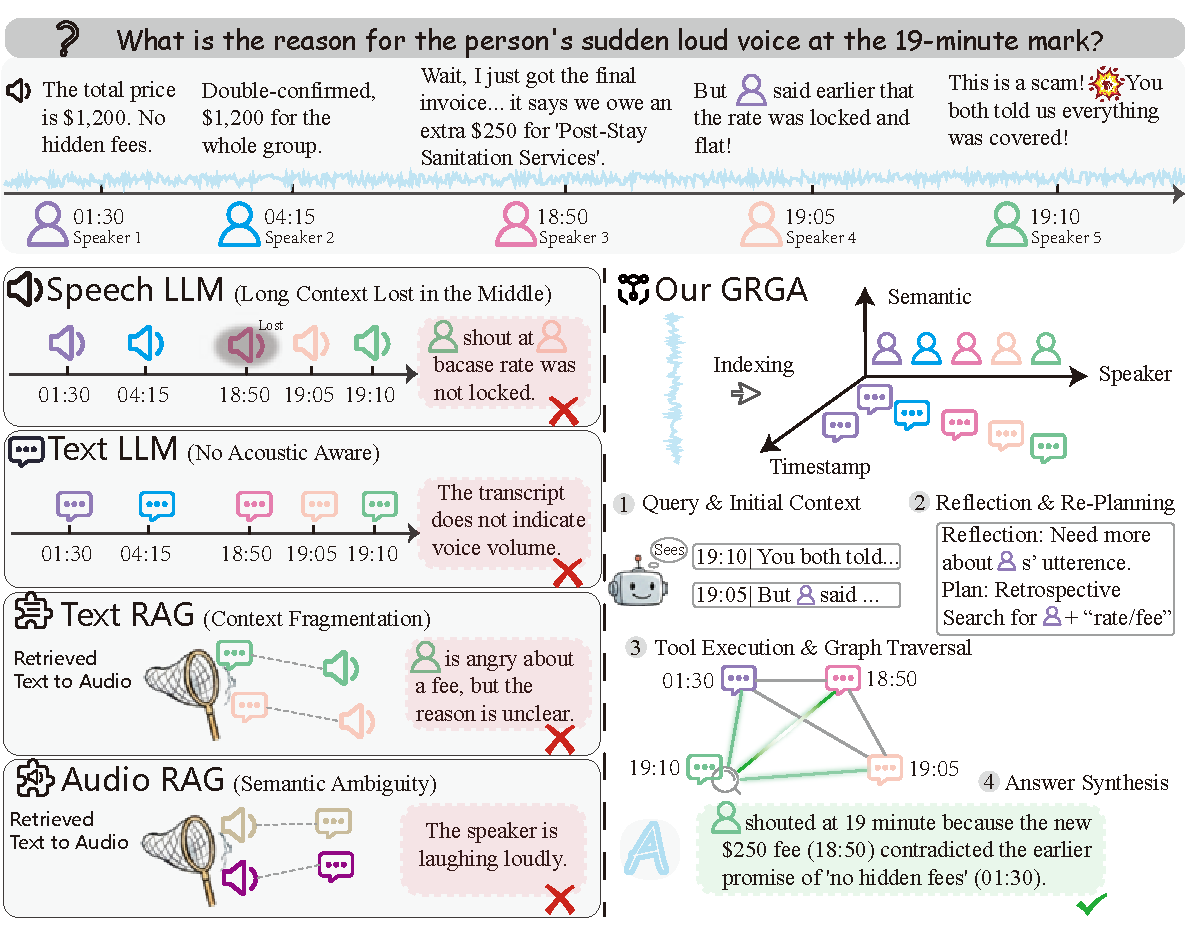
\includegraphics[width=0.96\linewidth]{figure/intro.pdf}
    \end{whitebox}
    % \vspace{0.25cm}
    % {\smallText\color{AppleGray}
    % GRGA indexes conversation along semantic, speaker, timestamp, and acoustic dimensions.}
  \end{posterbox}
\end{column}
\hspace{\columnGap}

\begin{column}{\wideColumn}
  \begin{posterbox}
    \sectionTitle{GRGA: Graph Retrieval + Planning}
    \begin{whitebox}
      \centering
      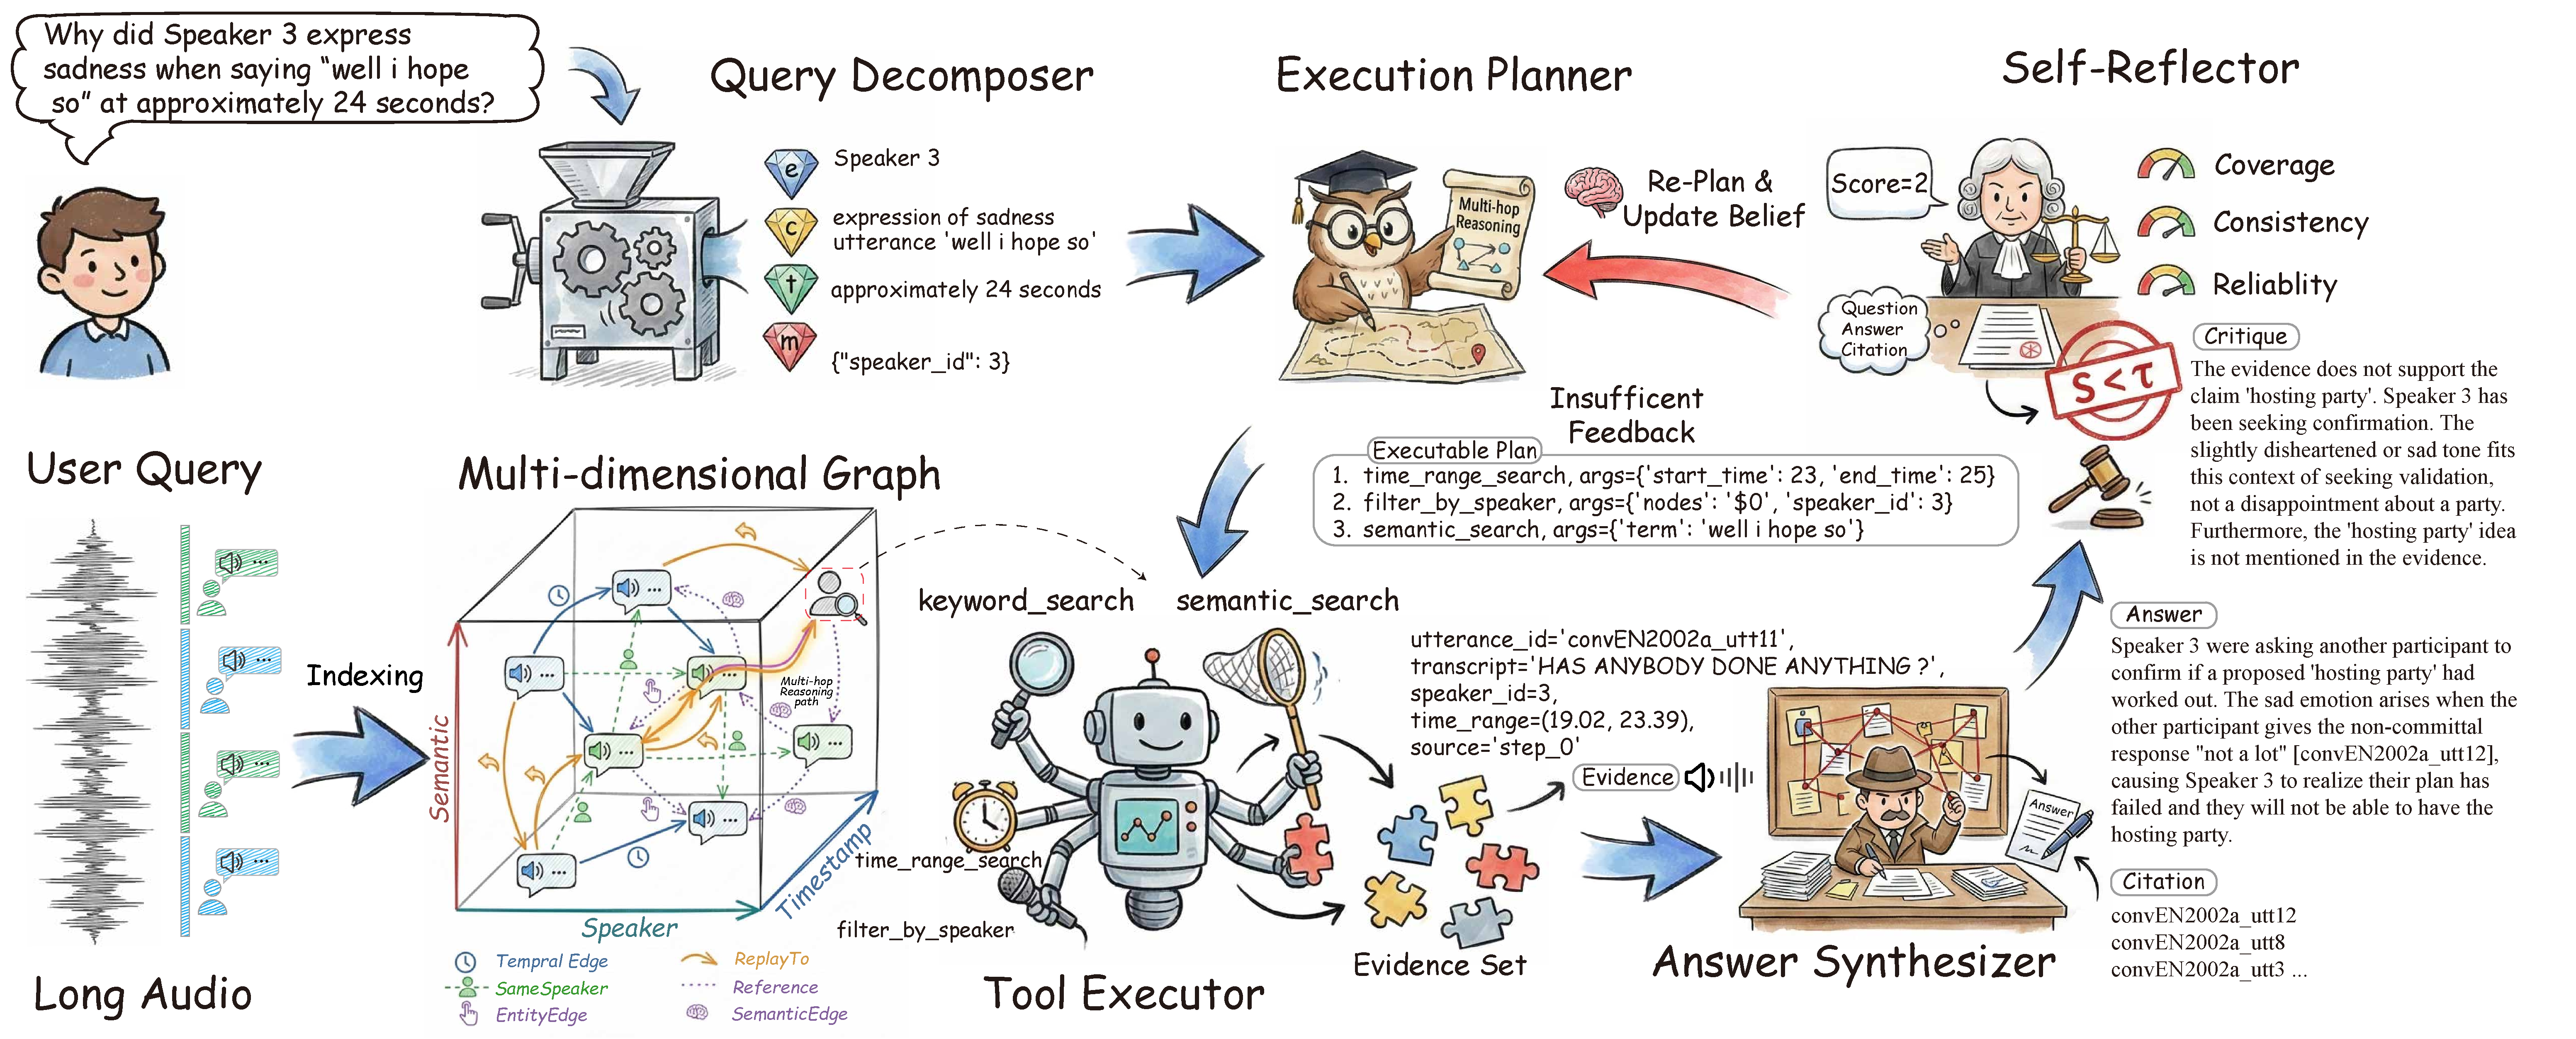
\includegraphics[width=0.98\linewidth]{figure/method.pdf}
    \end{whitebox}
    \vspace{0.2cm}
    \begin{posterlist}
      \item Audio is converted into utterance nodes with text, speaker, timestamps, and audio references.
      \item Edges encode temporal adjacency, reply-to relations, same-speaker links, entity co-occurrence, and semantic coreference.
      \item The agent decomposes each query, plans tool calls, executes graph retrieval, synthesizes an answer, then reflects for support.
    \end{posterlist}
  \end{posterbox}
\end{column}
\end{columns}
\end{postercontent}

\vspace{0.3cm}
\begin{postercontent}
\begin{columns}[t,totalwidth=\linewidth]

\begin{column}{\mainColumn}
  \begin{posterbox}
    \sectionTitle{LongAudioQA}
    \begin{posterlist}
      \item New QA dataset for long-form meeting and conversation understanding.
      \item Built from AliMeeting, AMI Meeting, and DailyTalk with human verification.
      \item Five skills: factual retrieval, inferential reasoning, temporal grounding, summarization, and acoustic-aware reasoning.
    \end{posterlist}
    \vspace{0.25cm}
    \begin{whitebox}
      \centering
      \begin{tabularx}{0.96\linewidth}{lrrrr}
        \toprule
        \textbf{Dataset} & \textbf{Dur(h)} & \textbf{Avg(s)} & \textbf{Turns} & \textbf{Q\&A} \\
        \midrule
        AliMeeting & 14.91 & 1,935 & 815 & 3,013 \\
        AMI        & 18.24 & 1,930 & 757 & 3,243 \\
        DailyTalk  & 21.59 & 610   & 186 & 10,200 \\
        \bottomrule
      \end{tabularx}
    \end{whitebox}
    \begin{whitebox}
      \centering
      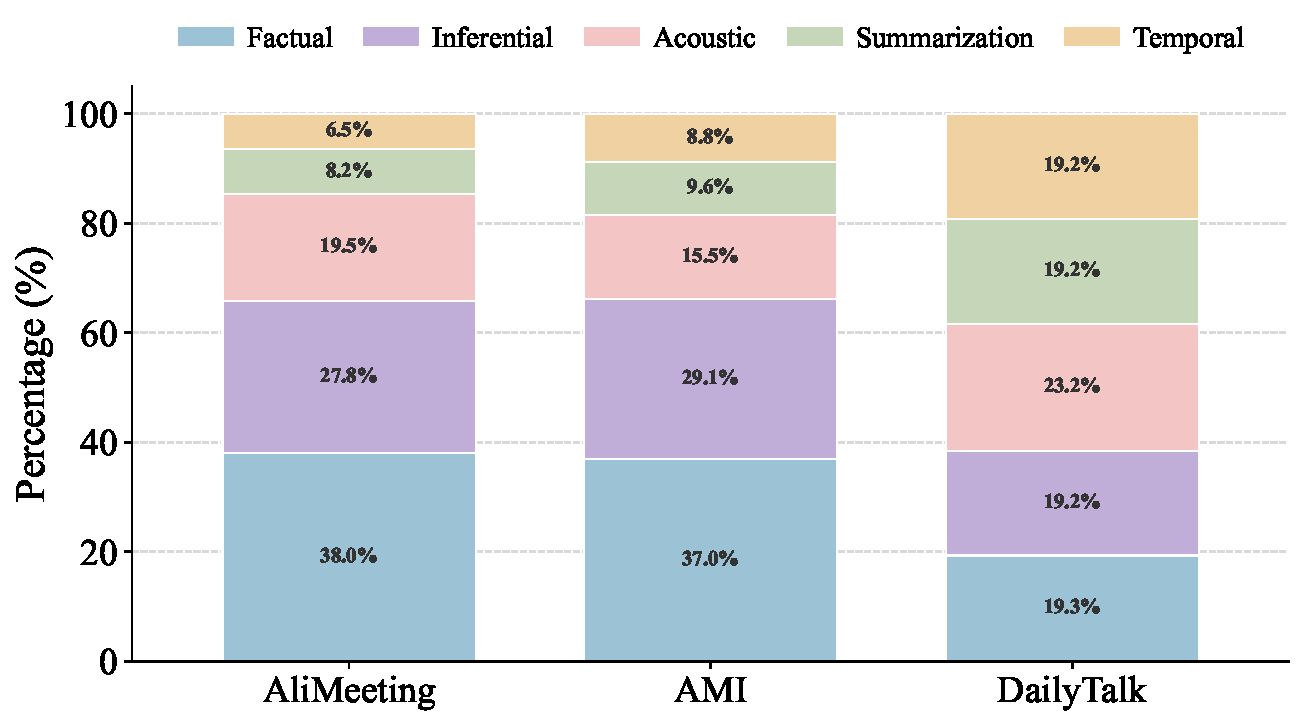
\includegraphics[width=0.78\linewidth]{figure/qa_distribution.pdf}
    \end{whitebox}
  \end{posterbox}

  \begin{posterbox}
    \sectionTitle{Question Taxonomy}
    \smallText
    \begin{tabularx}{\linewidth}{>{\bfseries}p{0.29\linewidth}Y}
      \toprule
      Factual & Entity retrieval, attribute association, keyword locating. \\
      Inferential & Multi-hop links between early problems, later discussions, and final decisions. \\
      Temporal & Absolute localization, relative sequencing, frequency statistics in time windows. \\
      Summarization & Topic consensus and speaker contribution aggregation. \\
      Acoustic-aware & Align emotion, intensity, laughter, or volume spikes with semantic context. \\
      \bottomrule
    \end{tabularx}
  \end{posterbox}

  \begin{posterbox}
    \sectionTitle{Robustness Under Noise}
    \begin{whitebox}
      \centering
      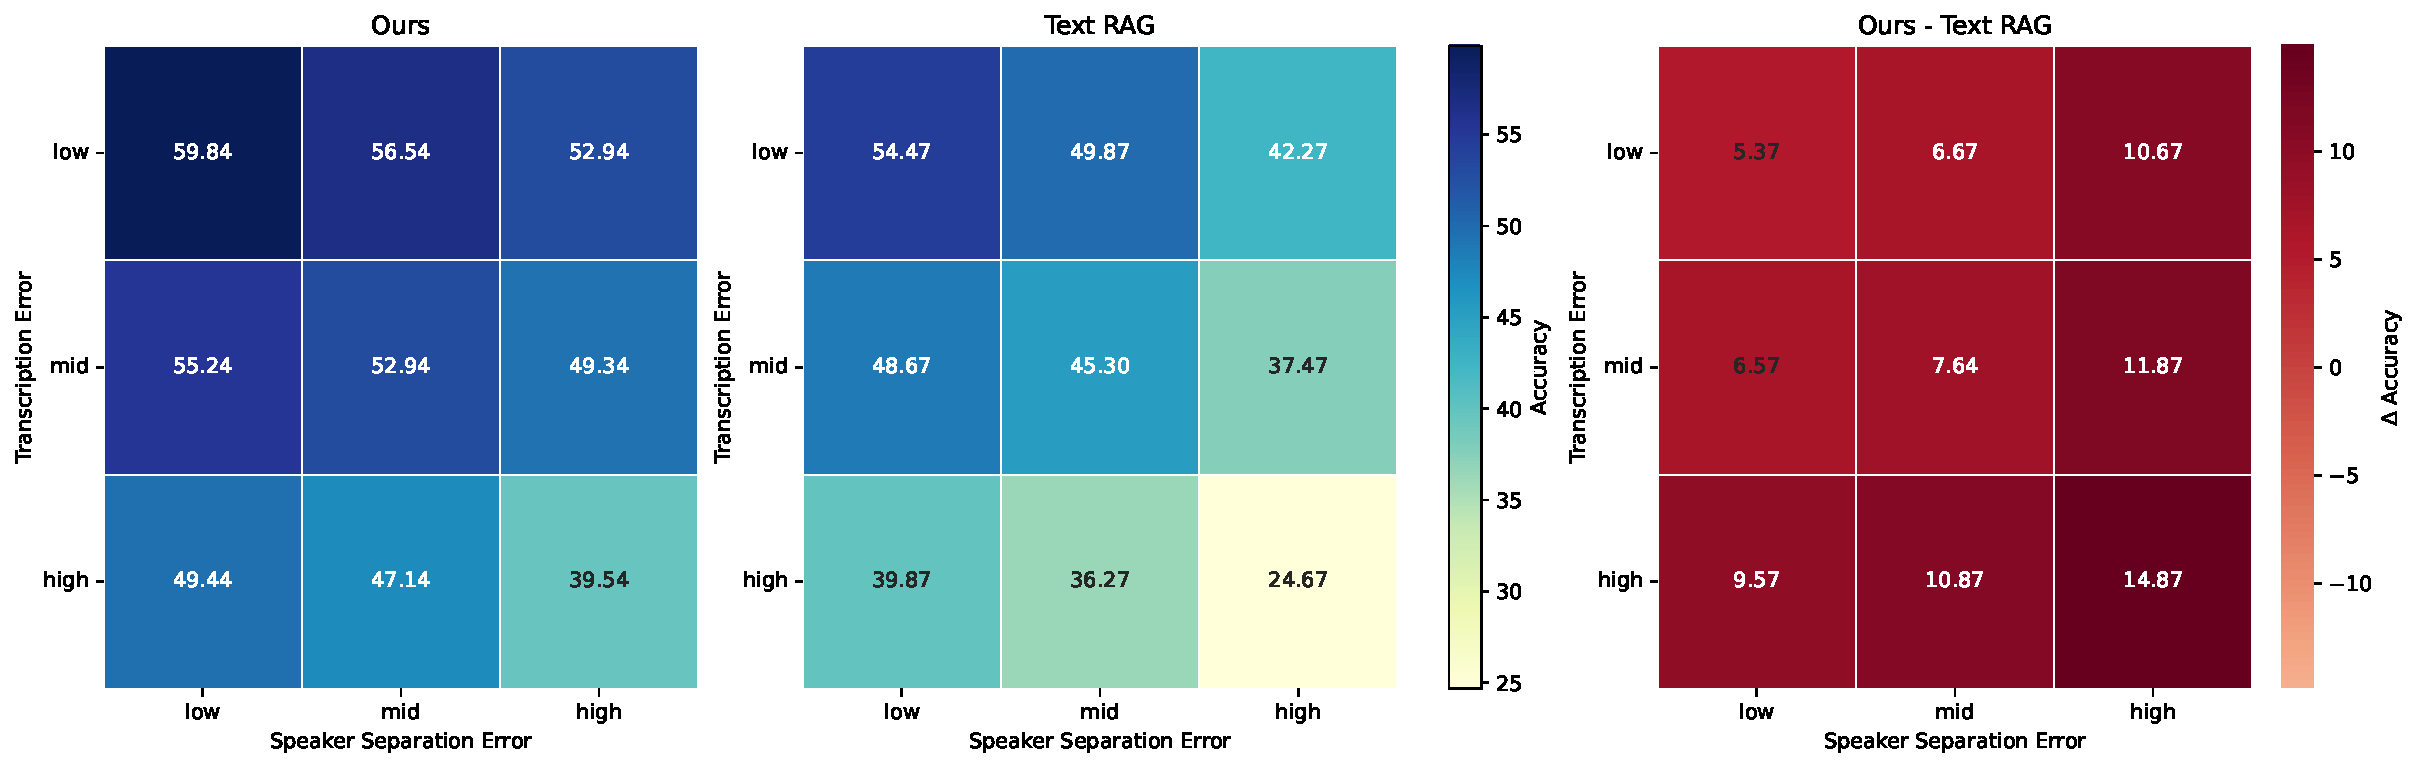
\includegraphics[width=0.96\linewidth]{figure/heatmaps_3panel.pdf}
    \end{whitebox}
    \begin{posterlist}
      \item Text RAG degrades sharply as ASR and diarization noise increase.
      \item GRGA acts as a structured noise buffer by validating evidence through graph links and reflection.
    \end{posterlist}
  \end{posterbox}

  \begin{posterbox}
    \sectionTitle{Conclusion}
    {\fontsize{28}{34}\selectfont\bfseries\color{AppleBlue}
    Long-form audio QA needs planning, not just listening.\par}
    \vspace{0.35cm}
    \begin{posterlist}
      \item \textbf{Dataset:} LongAudioQA introduces long-context, multi-speaker, temporal, and acoustic-aware QA.
      \item \textbf{Method:} GRGA turns meetings into multi-dimensional graphs and solves QA through tool-using agent planning.
      \item \textbf{Evidence:} Improvements appear in accuracy, citation precision/recall, human groundedness, and noisy settings.
    \end{posterlist}
  \end{posterbox}
\end{column}
\hspace{\columnGap}

\begin{column}{\mainColumn}

  \begin{posterbox}
    \sectionTitle{Reasoning Loop}
    \begin{center}
    \begin{tikzpicture}[
      node distance=0.74cm,
      flownode/.style={
        rounded corners=7pt,
        draw=AppleLine,
        fill=white,
        line width=0.6pt,
        minimum width=0.87\linewidth,
        minimum height=1.38cm,
        align=center,
        font=\fontsize{19}{23}\selectfont\bfseries
      },
      arrow/.style={-stealth,line width=1.1pt,color=AppleBlue}
    ]
      \node[flownode] (q) {1. Query Decomposition};
      \node[flownode,below=of q] (p) {2. Execution Planning};
      \node[flownode,below=of p] (e) {3. Graph Tool Execution};
      \node[flownode,below=of e] (s) {4. Citation-backed Synthesis};
      \node[flownode,below=of s] (r) {5. Self-Reflection};
      \draw[arrow] (q) -- (p);
      \draw[arrow] (p) -- (e);
      \draw[arrow] (e) -- (s);
      \draw[arrow] (s) -- (r);
      \draw[arrow] (r.east) to[out=0,in=0,looseness=1.45]
        node[pos=0.55,above left,font=\fontsize{15}{18}\selectfont\color{AppleGray}]{re-plan}
        (p.east);
    \end{tikzpicture}
    \end{center}
    \vspace{0.2cm}
    \begin{whitebox}
      \miniTitle{Action Space}
      \vspace{0.25cm}
      \smallText
      \pill{AppleBlue}{Semantic Search}
      \hspace{0.12cm}
      \pill{AppleGreen}{Graph Traversal}
      \hspace{0.12cm}
      \pill{AppleOrange}{Filtering}
      \hspace{0.12cm}
      \pill{AppleRed}{Audio Access}
    \end{whitebox}
  \end{posterbox}

  \begin{posterbox}
    \sectionTitle{Why Planning Helps}
    \begin{whitebox}
      \centering
      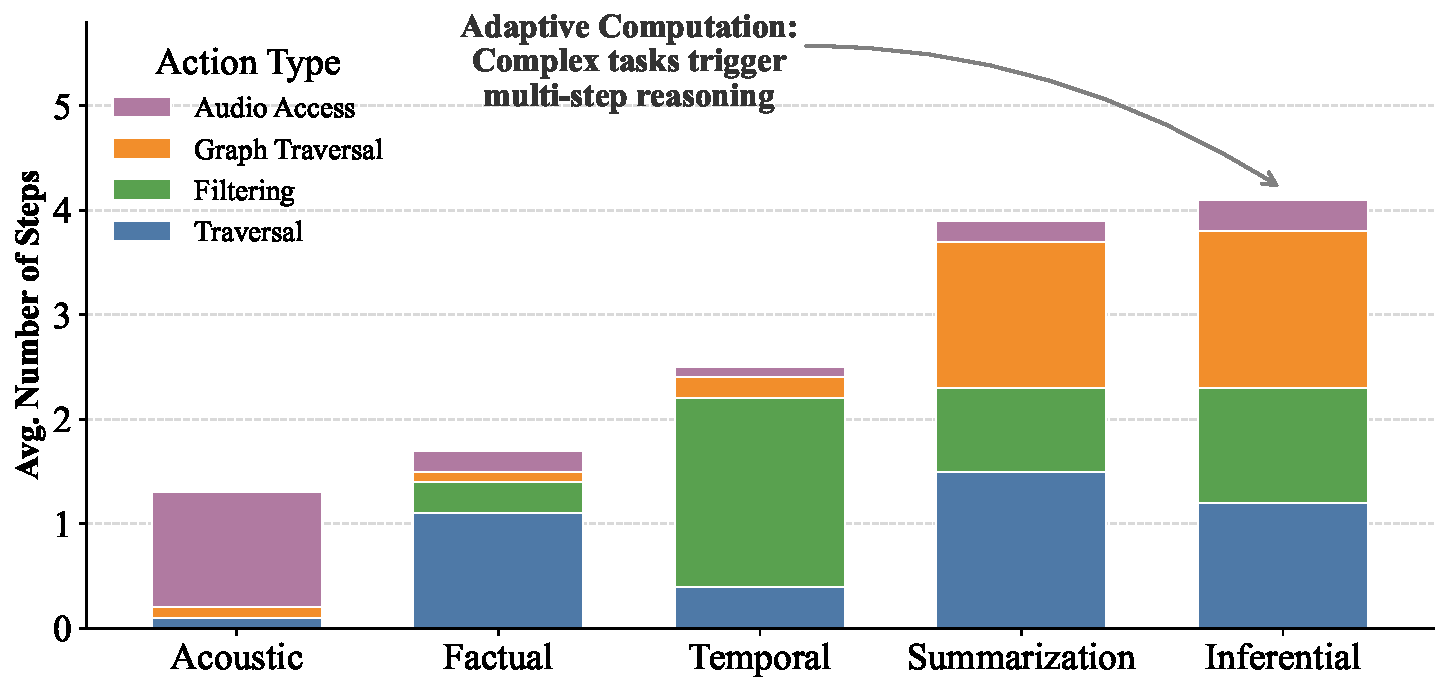
\includegraphics[width=0.93\linewidth]{figure/step_analysis.pdf}
    \end{whitebox}
    \begin{posterlist}
      \item Factual queries can terminate quickly with semantic search.
      \item Inferential and temporal questions trigger deeper graph traversal.
      \item Acoustic-aware questions selectively access raw audio when transcripts are insufficient.
    \end{posterlist}
  \end{posterbox}

  \begin{posterbox}
    \sectionTitle{Self-Correction Case}
    \begin{whitebox}
      \smallText
      \textbf{Query:} ``What is the team's general attitude to the project deadline and workload?''\par
      \vspace{0.35cm}
      \begin{tabularx}{\linewidth}{>{\bfseries}p{0.24\linewidth}Y}
        \toprule
        Initial answer & Generic summary: the deadline is tight and members feel urgency. \\
        Reflection & Low confidence; needs concrete evidence for ``tight'' and ``work-intensive''. \\
        Re-plan & Search for deadline and workload sentiment; retrieve specific utterances. \\
        Final answer & Cites ``six days'', ``change the deadlines'', ``a hassle'', and ``superficially''. \\
        \bottomrule
      \end{tabularx}
    \end{whitebox}
    \begin{posterlist}
      \item Reflection converts unsupported fluent text into evidence-seeking behavior.
      \item Final response is anchored to exact utterance-level citations.
    \end{posterlist}
  \end{posterbox}

  \begin{posterbox}
    \sectionTitle{Ablation Highlights}
    \smallText
    \begin{tabularx}{\linewidth}{Ycc}
      \toprule
      \textbf{Removed Component} & \textbf{Avg.} & \textbf{Drop} \\
      \midrule
      Full GRGA & \textbf{49.49} & -- \\
      w/o Reflection & 39.64 & -9.84 \\
      w/o Graph Traversal & 38.21 & -11.27 \\
      w/o Audio Access & 34.71 & -14.78 \\
      w/o Semantic Search & 16.28 & -33.21 \\
      \bottomrule
    \end{tabularx}
    \vspace{0.35cm}
    \begin{posterlist}
      \item Semantic search finds entry evidence; graph traversal connects dispersed clues.
      \item Audio access is crucial for acoustic-aware questions.
      \item Reflection prevents accepting unsupported first-pass answers.
    \end{posterlist}
  \end{posterbox}
\end{column}
\hspace{\columnGap}

\begin{column}{\mainColumn}
  \begin{posterbox}
    \sectionTitle{Main Results}
    \begin{columns}[T,totalwidth=\linewidth]
      \begin{column}{0.32\linewidth}
        \metricCard{AppleBlue}{+40.7}{AMI Inferential\\vs Text RAG}
      \end{column}
      \begin{column}{0.32\linewidth}
        \metricCard{AppleGreen}{52.32}{DailyTalk Acoustic\\accuracy}
      \end{column}
      \begin{column}{0.32\linewidth}
        \metricCard{AppleOrange}{61.10}{DailyTalk Summarization\\accuracy}
      \end{column}
    \end{columns}
    \vspace{0.3cm}
    \begin{whitebox}
      \centering
      \tinyPoster
      \setlength{\tabcolsep}{3.2pt}
      \begin{tabular}{lccccc}
        \toprule
        \textbf{AMI Method} & \textbf{Fact.} & \textbf{Infer.} & \textbf{Temp.} & \textbf{Summ.} & \textbf{Acou.} \\
        \midrule
        Qwen3-Omni speech & 20.96 & 26.38 & 15.12 & 16.67 & 12.15 \\
        MiMo-Audio text & 53.62 & 44.10 & 37.14 & 41.49 & 17.94 \\
        BGE-M3 Text RAG & 32.56 & 24.56 & 23.78 & 25.36 & 25.34 \\
        CLASP Audio RAG & 24.12 & 20.31 & 22.76 & 11.60 & 14.79 \\
        \rowcolor{AppleLight}
        \textbf{GRGA} & \textbf{59.46} & \textbf{65.29} & \textbf{38.56} & \textbf{48.46} & \textbf{35.68} \\
        \bottomrule
      \end{tabular}
    \end{whitebox}
    \smallText\color{AppleGray}
    Semantic Accuracy (\%) with LLM-as-a-judge. GRGA is best across all AMI question types.
  \end{posterbox}

  \begin{posterbox}
    \sectionTitle{Grounded Answers}
    \begin{whitebox}
      \centering
      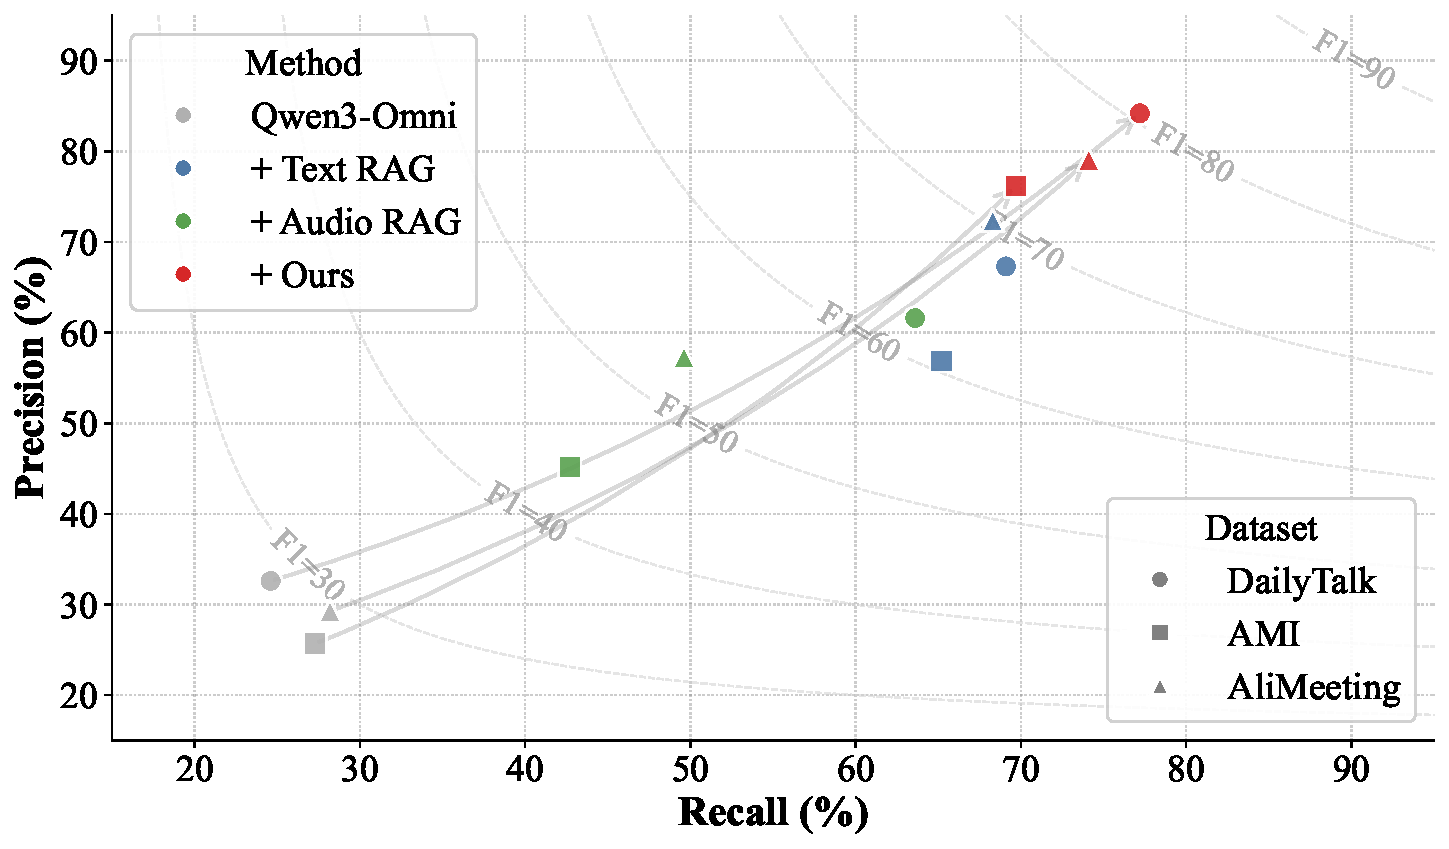
\includegraphics[width=0.96\linewidth]{figure/pr_scatter.pdf}
    \end{whitebox}
    \vspace{0.25cm}
    \begin{whitebox}
      \centering
      \smallText
      \begin{tabular}{lcc}
        \toprule
        \textbf{Method on AMI} & \textbf{Precision} & \textbf{Recall} \\
        \midrule
        Qwen3-Omni & 25.7 & 27.3 \\
        + Text RAG & 56.9 & 65.2 \\
        + Audio RAG & 45.2 & 42.7 \\
        \rowcolor{AppleLight}
        \textbf{+ GRGA} & \textbf{76.2} & \textbf{69.7} \\
        \bottomrule
      \end{tabular}
    \end{whitebox}
    {\smallText\color{AppleGray}Citation accuracy uses a $\pm 2$s tolerance over timestamp evidence.}
  \end{posterbox}

  \begin{posterbox}
    \sectionTitle{Human Evaluation}
    \begin{whitebox}
      \centering
      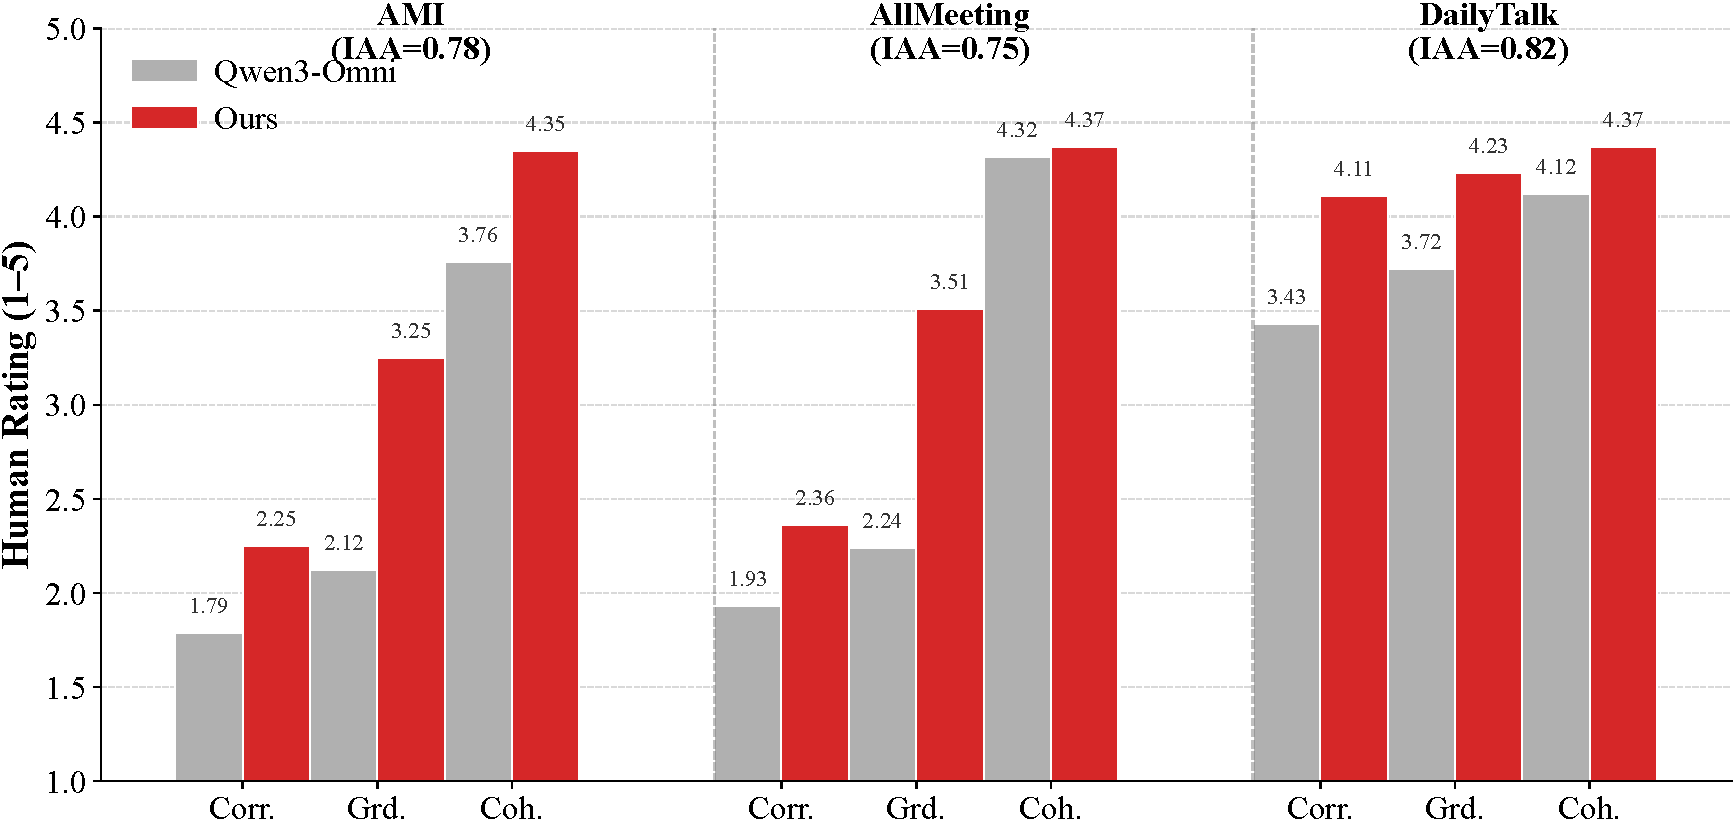
\includegraphics[width=0.94\linewidth]{figure/human_eval.pdf}
    \end{whitebox}
    \begin{columns}[T,totalwidth=\linewidth]
      \begin{column}{0.48\linewidth}
        \metricCard{AppleGreen}{+0.97}{Overall groundedness gain}
      \end{column}
      \begin{column}{0.48\linewidth}
        \metricCard{AppleBlue}{+0.52}{Overall correctness gain}
      \end{column}
    \end{columns}
  \end{posterbox}

\end{column}
\end{columns}
\end{postercontent}

\vfill
\begin{postercontent}
  {\fontsize{17}{21}\selectfont\color{AppleGray}
  ACL 2026 Poster \quad | \quad LongAudioQA and GRGA \quad | \quad Corresponding author: Dong Zhang
  \hfill
  Code/Data: github.com/tangquanwei/GRGA\par}
\end{postercontent}
\vspace*{0.35cm}

\end{frame}
\end{document}
